\chapter{Partial Differential Equations}\label{ch:PDEs}

This brief document contains class notes, explanations, examples, and problems for our
brief introduction to partial differential equations (PDEs).  The study of PDEs spans all
fields of the mathematical sciences, and like ODEs, PDEs are the language used by
scientists to model change.  The change this time happens simultaneously in all three
spatial dimensions as well as time.


\section{Some Reminders from Multivariable Calculus}
\begin{problem}
    Let $f(x,y)$ be a differentiable multivariable function.  Which of the following is
    the gradient of $f$?
    \begin{itemize}
        \item[(a)] $\displaystyle \nabla f = \left< \pd{f}{y} \, , \, \pd{f}{x} \right>$
        \item[(b)] $\displaystyle \nabla f = \pd{f}{x} + \pd{f}{y}$
        \item[(c)] $\displaystyle \nabla f = \left< \pd{f}{x} \, , \, \pd{f}{y} \right>$
        \item[(d)] $\displaystyle \nabla f = \pdd{f}{x} + \pdd{f}{y}$
    \end{itemize}
\end{problem}

\begin{problem}
    Let $\mathcal{F}(x,y)$ be a vector function so that 
    \[ \mathcal{F}(x,y) = \left< f_1(x,y) \, , \, f_2(x,y) \right>. \]
    Which of the following is the divergences of $\mathcal{F}$?
    \begin{itemize}
        \item[(a)] $\displaystyle \nabla \cdot \mathcal{F} = \pd{f_1}{x} + \pd{f_2}{y}$
        \item[(b)] $\displaystyle \nabla \cdot \mathcal{F} = \pdd{f_1}{x} + \pdd{f_2}{y}$
        \item[(c)] $\displaystyle \nabla \cdot \mathcal{F} = \left< \pd{f_1}{y} +
            \pd{f_2}{x} \, , \, \pd{f_1}{x} + \pd{f_2}{y} \right>$
        \item[(d)] $\displaystyle \nabla \cdot \mathcal{F} = \left< \pd{f_1}{x} \, , \,
            \pd{f_2}{y} \right>$
    \end{itemize}
\end{problem}

\begin{problem}
    Let $f(x,y)$ be a twice differentiable function.  Which of the following is the result
    of taking the divergence of the gradient of $f$?
    \begin{itemize}
        \item[(a)] $\displaystyle \nabla \cdot \nabla f = \pd{f}{x} + \pd{f}{y}$
        \item[(b)] $\displaystyle \nabla \cdot \nabla f = \pdd{f}{x} + \pdd{f}{y}$
        \item[(c)] $\displaystyle \nabla \cdot \nabla f = \left< \pdd{f}{x} ,  \pdd{f}{y}
            \right>$
        \item[(d)] $\displaystyle \nabla \cdot \nabla f = \left< \pd{f}{x} , \pd{f}{y}
            \right>$
    \end{itemize}
\end{problem}

\begin{problem}
    The last quarter of multivariable calculus contains some beautiful properties from
    vector calculus.  Of particular interest here is the divergence theorem:
    \[ \iint \bq \cdot n dA = \iiint \nabla \cdot \bq dV. \]
    In words, this theorem says
    \begin{itemize}
        \item[(a)] The flux of a vector field $\bq$ through the surface of an object is
            equal to how the vector  field $\bq$ spreads out within the object.
        \item[(b)] The amount of work done by the vector field $\bq$ is equal to how the
            vector field $\bq$ curls within the object.
        \item[(c)] The amount of work gained or lost by traveling around the exterior of
            the object is equal to the amount that the vector field $\bq$ spreads out
            within the object.
        \item[(d)] The flux of a vector field $\bq$ through the surface of an object is
            equal to how the vector field $\bq$ curls within the object.
    \end{itemize}
\end{problem}

\begin{problem}
    The heat equation (which we will derive in a bit) is 
    \[ \pd{u}{t} = k \nabla \cdot \nabla u. \]
    If $u(x,y,z,t)$ is the temperature of an object then what does the heat equation say
    in words?
\end{problem}


\newpage\section{Where to PDEs Come From?}
This somewhat lengthy section is meant to be an introduction to many of the primary
partial differential equations of interest in basic mathematical physics.
    
We start with a brief derivation of a {\it general conservation law}.  The result
being a partial differential equation that can be used for conservation of mass,
momentum, or energy.
Let $u$ be the quantity you are trying to conserve, $\bq$ be the flux of that quantity,
and $f$ be any source of that quantity.  For example, if we are to derive a conservation
of energy equation, $u$ might be energy, $\bq$ might be temperature flux, and $f$ might be
a temperature source (or sink).

\subsection{Derivation of General Balance Law}
Let $\Omega$ be a fixed volume and denote the boundary of this volume by $\partial
\Omega$. The rate at which $u$ is changing in time throughout $\Omega$ needs to be
balanced by the rate at which $u$ leaves the volume plus any sources of $u$.
Mathematically, this means that
\begin{flalign}
    \pd{ }{t} \iiint_{\Omega} u dV = -\iint_{\partial \Omega} \bq \cdot n dA +
    \iiint_\Omega f dV.
    \label{eqn:global_balance}
\end{flalign}
This is a global balance law in the sense that it holds for all volumes $\Omega$.  The
troubles here are two fold: (1) there are many integrals, and (2) there are really two variables
($u$ and $q$ since $f=f(u,x,t)$) so the equation is not closed.  In order to mitigate
that fact we apply the divergence theorem to get
\begin{flalign}
    \pd{ }{t} \iiint_{\Omega} u dV = -\iiint_{\Omega} \nabla \cdot \bq dV +
    \iiint_\Omega f dV.
    \label{eqn:global_balance2}
\end{flalign}

Gathering all of the terms on the right of \eqref{eqn:global_balance2}, interchanging the
integral and the derivative on the left (since the volume is not changing in time), and
rewriting gives
\begin{flalign}
    \iiint_\Omega \left( \pd{u}{t} + \nabla \cdot \bq \right) dV = \iiint_\Omega f dV
    \label{eqn:global_balance3}
\end{flalign}
If we presume that this equation holds for all volumes $\Omega$ then the integrands must
be equal and we get the local balance law
\begin{flalign}
    \boxed{\pd{u}{t} + \nabla \cdot \bq = f.}
    \label{eqn:local_balance}
\end{flalign}
In particular, the physics of energy, momentum, and mass transport are governed by
\eqref{eqn:local_balance}.  In each of these instances we need to have a suitable
functional form of the flux $\bq$.  In the following subsection we will discuss one common
form of $\bq$.

\subsection{Simplifications of the Local Balance Law}
If equation \eqref{eqn:local_balance} it is often assumed that the system is free of
external sources.  In this case we set $f$ to zero and obtain the source-free balance law
\begin{flalign}
    \pd{u}{t} + \nabla \cdot \bq = 0.
    \label{eqn:local_source_free}
\end{flalign}
It is this form of balance law where many of the most interesting and important partial
differential equations come from.  In particular consider the following two cases: mass
balance and energy balance.
\subsubsection{Mass Balance}
In mass balance we take $u$ to either be the density of a substance (e.g. in the case of
liquids) or the concentration of a substance in a mixture (e.g. in the case of
gasses). If $C$ is the mass concentration of a substance in a gas then the flux of that
substance is given via Fick's Law as
\begin{flalign}
    \bq = -k \nabla C.
    \label{eqn:fick}
\end{flalign}
Combining \eqref{eqn:fick} with \eqref{eqn:local_source_free} (and assuming that $k$ is
independent of space, time, and concentration) gives
\begin{flalign}
    \pd{C}{t} = k \nabla \cdot \nabla C. 
    \label{eqn:fick2_simp}
\end{flalign}
In the presenence of external sources of mass, \eqref{eqn:fick2_simp} is
\begin{flalign}
    \pd{C}{t} = k \nabla \cdot \nabla C + f(x).
    \label{eqn:fick3}
\end{flalign}
\begin{problem}
    What does \eqref{eqn:fick3} equation look like in terms of spatial derivatives on the
    right-hand side?
    \begin{flalign*}
        \pd{C}{t} &= \underline{\hspace{2in}} \quad \text{(1 Spatial Dimension)} \\
        \pd{C}{t} &= \underline{\hspace{2in}} \quad \text{(2 Spatial Dimensions)} \\
        \pd{C}{t} &= \underline{\hspace{2in}} \quad \text{(3 Spatial Dimensions)}
    \end{flalign*}
\end{problem}

\subsubsection{Energy Balance}
The energy balance equation is essentially the same as the mass balance equation.  If $u$
is temperature then the flux of temperature is given by Fourier's Law for heat conduction
\begin{flalign}
    q = -k\nabla T.
    \label{eqn:fourier}
\end{flalign}
Making the same simplifications as in the mass balance equation we arrive at
\begin{flalign}
    \pd{T}{t} = k \nabla \cdot \nabla T.
    \label{eqn:fourier2}
\end{flalign}
In the presence of external sources of heat, \eqref{eqn:fourier2} becomes
\begin{flalign}
    \pd{T}{t} = k \nabla \cdot \nabla T + f(x).
    \label{eqn:fourier3}
\end{flalign}
\begin{problem}
    What does \eqref{eqn:fourier3} equation look like in terms of spatial derivatives on the
    right-hand side?
    \begin{flalign*}
        \pd{T}{t} &= \underline{\hspace{2in}} \quad \text{(1 Spatial Dimension)} \\
        \pd{T}{t} &= \underline{\hspace{2in}} \quad \text{(2 Spatial Dimensions)}\\
        \pd{T}{t} &= \underline{\hspace{2in}} \quad \text{(3 Spatial Dimensions)}
    \end{flalign*}
\end{problem}


\subsection{Laplace's Equation and Poisson's Equation}
Equations \eqref{eqn:fick3} and \eqref{eqn:fourier3} are the same partial differential
equation for two very important physical phenomenon; mass and heat transfer.  In the case
where time is allowed to run to infinity and no external sources of mass or energy are
included these equations reach a steady state solution (no longer changing in time) and we
arrive at Laplace's Equation
\begin{flalign}
    \nabla \cdot \nabla u = 0.
    \label{eqn:laplace}
\end{flalign}
Laplace's equation is actually a statement of minimal energy as well as steady state heat
or temperature.  We can see this since entropy always drives systems from high energy to
low energy, and if we have reached a steady state then we must have also reached a surface
of minimal energy.

\begin{problem}
    Equation \eqref{eqn:laplace} is sometimes denoted as $\nabla \cdot \nabla u = \nabla^2 u =
    \Delta u$, and in terms of the partial derivatives it is written as
    \begin{flalign*}
        0 &= \underline{\hspace{2in}} \quad \text{(1 Spatial Dimension)} \\
        0 &= \underline{\hspace{2in}} \quad \text{(2 Spatial Dimensions)} \\
        0 &= \underline{\hspace{2in}} \quad \text{(3 Spatial Dimensions)} 
    \end{flalign*}
\end{problem}

If there is a time-independent external source the the right-hand side of
\eqref{eqn:laplace} will be non-zero and we arrive at Poisson's equation:
\begin{flalign}
    \nabla \cdot \nabla u = -f(x).
    \label{eqn:poisson}
\end{flalign}
Note that the negative on the right-hand side comes from the fact that
$\pd{u}{t} = k \nabla \cdot \nabla u + f(x)$ and $\pd{u}{t} \to 0$.  Technically we are
taking absorbing the constant $k$ into $f$ (that is ``$f$'' is really ``$f/k$'').  Also
note that in many instances the value of $k$ is not contant and cannot therefore be pulled
out of the derivative without a use of the product rule.

We will start our exploration of numerical PDEs with Laplace's and Poisson's equations.
We will then layer on the temporal derivatives to explore mass and heat transport.
Finally, we will explore wave phenomena as well as advection-diffusion transport models.

\newpage\section{The 1D Heat Equation}
In this section we will discuss analytic techniques for solving the heat equation in 1
spatial dimension.  Most of this section is paraphrased from Richard Haberman's {\it Applied
Partial Differential Equations} text \cite{Haberman}.  

We can think of the heat equation physically as tracking the heat diffusion in a
thin rod of length $L$.  Hence, in 1 spatial dimension equation \eqref{eqn:fourier2}
becomes 
\begin{flalign}
    \pd{u}{t} &= k \pdd{u}{x} \quad
    \text{with } 0 < x < L \text{ and } t>0. \label{eqn:1Dheat} 
\end{flalign}
\begin{figure}[ht!]
    \begin{center}
        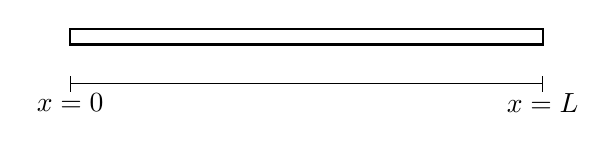
\begin{tikzpicture}
            \draw[thick, black] (0,0) -- (6,0) -- (6,0.2) -- (0,0.2) -- cycle;
            \draw[|-|] (0,-0.5) node[anchor=north]{$x=0$} -- (6,-0.5)
            node[anchor=north]{$x=L$};
        \end{tikzpicture}
    \end{center}
    \caption{Sample geometry for the 1D heat equation \eqref{eqn:1Dheat}.}
    \label{fig:1Dheat_rod}
\end{figure}

In each of the subsequent subsections of this document we will explore different boundary
conditions for equation \eqref{eqn:1Dheat}.  The boundary conditions are a way to
prescribe how the heat is transfering or is otherwise being controlled at the ends of the
rod.

\subsection{1D Heat Equation with Zero Temperature Ends}
For our first case, consider a 1D rod as in Figure \ref{fig:1Dheat_rod} with $u(0,t) = 0$
and $u(L,t) = 0$.  That is, let's assume that the two ends of the rod are in an ice bath
held at exactly $0^\circ$ (See Figure \ref{fig:1Dheat_rod_Dirichlet}).
\begin{figure}[ht!]
    \begin{center}
        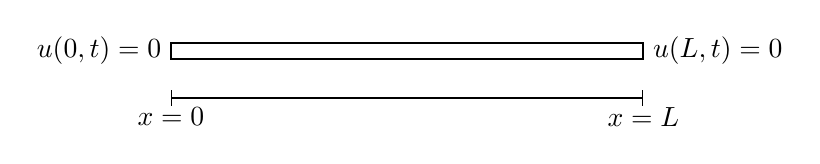
\begin{tikzpicture}
            \draw[thick, black] (0,0) -- (6,0) -- (6,0.2) -- (0,0.2) -- cycle;
            \draw[|-|] (0,-0.5) node[anchor=north]{$x=0$} -- (6,-0.5)
            node[anchor=north]{$x=L$};
            \draw (0,0.1) node[anchor=east]{$u(0,t)=0$};
            \draw (6,0.1) node[anchor=west]{$u(L,t)=0$};
        \end{tikzpicture}
    \end{center}
    \caption{Sample geometry for the 1D heat equation \eqref{eqn:1Dheat}.}
    \label{fig:1Dheat_rod_Dirichlet}
\end{figure}


\begin{problem}
    If we were to solve the 1D heat equation
    \[ \pd{u}{t} = k \pdd{u}{x} \]
    with boundary conditions as in Figure \ref{fig:1Dheat_rod_Dirichlet}, what other
    information would we need, aside from $k$, in order to get a physically meaningful
    solution?
    \begin{itemize}
        \item[(a)] $u(L/2,t)$: a fixed temperature at the midpoint
        \item[(b)] $u(x,0)$: an initial temperature profile along the rod
        \item[(c)] $u(x,\infty)$: the steady state temperature profile
        \item[(d)] $u(0,t)$: the way that the heat evolves at $x=0$
    \end{itemize}
\end{problem}

\begin{problem}
    Assume that $u(x,0) = 100$.  That is, assume that the rod is initially heated to
    $100^\circ$ from end to end.  Further assume that the boundary conditions are $u(0,t)
    = u(L,0) = 0$ just as in Figure \ref{fig:1Dheat_rod_Dirichlet}.  Draw several curves
    clearly showing how the temperature in the rod will evolve in time.  
\end{problem}

\subsubsection{Separation of Variables}
With ordinary differential equation we origianlly saw separation of variables with
relatively {\it simple} differential equations.  It turns out that we can do the same
thing the heat equation.  We start by assuming that in order to solve $\pd{u}{t} = k
\pdd{u}{x}$ we assume that 
\begin{flalign}
    u(x,t) &= \phi(x) G(t)
    \label{eqn:separation1}
\end{flalign}
where $\phi(x)$ is ONLY a function of space ($x$) and $G(t)$ is ONLY a function of time
($t$).  This technique was invented in the 1700's, and it works becuase it reduces the PDE
to two ODEs.

\begin{problem}
    Let's see what happens under assumption \eqref{eqn:separation1}:\\ Let $u(x,t) =
    \phi(x) G(t)$ and 
    \begin{itemize}
        \item write $\displaystyle \pd{u}{t}$ in terms of the functions $\phi$ and $G$,
        \item write $\displaystyle \pdd{u}{x}$ in terms of the functions $\phi$ and $G$,
            and 
        \item put your two answers into the heat equation $\displaystyle \pd{u}{t} = k
            \pdd{u}{x}$.
        \item Finally, separate the variables so that all of the expressions with $G$ are
            on the left of the equation and all of the expressions with $\phi$ are on the
            right of the equation. (put the $k$ with the $G$ function \dots trust me)
    \end{itemize}
\end{problem}

The left-hand side of your result from the previous problem should only contain function
of $G$ and the right-hand side should only contain functions of $\phi$.  The strange thing
is that the equal sign is still valid.  How can this be?  The left-hand side is only a function
of $t$ and the right-hand side is only a function of $x$.
\begin{problem}
    From the previous question you should have arrived at
    \[ \frac{1}{kG} \frac{dG}{dt} = \frac{1}{\phi} \frac{d^2 \phi}{dx^2}. \]
    The left-hand side is only a function of $t$ and the right-hand side is only a
    function $x$ but the equal sign is absolutely true for all $x$ and for all $t$.  How
    can this be?
\end{problem}

\begin{problem}
    From the separation of variables we arrive at two ordinary differential equations:
    \begin{flalign}
        \frac{d^2 \phi}{dx^2} &= -\lambda \phi 
        \label{eqn:separation_space} \\
        \frac{dG}{dt} &= -\lambda k G.
        \label{eqn:separation_time}
    \end{flalign}
    What types of behavior do you expect out of the solutions for equations
    \eqref{eqn:separation_space} and \eqref{eqn:separation_time}. 
    \begin{itemize}
        \item[(a)] Equation \eqref{eqn:separation_space}: exponential decay \\
            Equation \eqref{eqn:separation_time}: oscillations modeled by trig functions
        \item[(b)] Equation \eqref{eqn:separation_space}: over damped system modeled by
            exponential functions \\
            Equation \eqref{eqn:separation_time}: exponential decay
        \item[(c)] Equation \eqref{eqn:separation_space}: critically damped system modeled by
            exponential functions \\
            Equation \eqref{eqn:separation_time}: exponential decay
        \item[(d)] Equation \eqref{eqn:separation_space}: oscillations modeled by trig
            functions \\
            Equation \eqref{eqn:separation_time}: exponential decay
    \end{itemize}
\end{problem}

\begin{problem}\label{prob:separation_ivp}
    Solve the time-dependent equation 
    \[ \frac{dG}{dt} = -\lambda k G \]
    where $\lambda$ is (at the moment) an unknown constant. What happens if $\lambda>0$,
    if $\lambda = 0$, and if $\lambda <0$?
\end{problem}

Note: We don't expect to have solutions that grow exponentially in time so we should
expect that $\lambda \ge 0$

\begin{problem}\label{prob:separation_bvp}
    Now we're going to solve the spatial boundary-valued problem
    \[ \frac{d^2\phi}{dx^2} = -\lambda \phi \quad \text{with} \quad \phi(0) = 0 \text{ and
    } \phi(L) = 0. \]
    \begin{itemize}
        \item Assume that $\phi(x) = e^{rx}$, find the characteristic polynomial, and find
            the two linearly independent solutions (these will contain $\lambda$).
        \item Write the solution to $\phi$ as a linear combination of the two linearly
            independent solutions.
        \item Apply the left-hand boundary condition $\phi(0) = 0$ to get one of the
            constants.
        \item Apply the right-hand boundary condition $\phi(L) = 0$ and find the equation
            that must be true in order for this boundary condition to be satisfied.
        \item What must $\lambda$ be equal to in order for the previous equation to be
            satisfied?
        \item Write the solution to $\phi(x)$.
    \end{itemize}
\end{problem}

Let me interject here for a few sentences:\\
Let's put the pieces together.  From Problem \ref{prob:separation_ivp} we know that 
\begin{flalign}
    G(t) = C_1 e^{-\lambda k t} 
\end{flalign}
and from Problem \ref{prob:separation_bvp} we know that 
\begin{flalign}
    \phi(x) = C_2 \sin \left( \frac{n \pi x}{L} \right).
\end{flalign}
Since we are assuming that $u(x,t) = \phi(x) G(t)$ we can multiply the time dependent
solution $G(t)$ and the spatial solution $\phi(x)$ to get
\begin{flalign}
    u(x,t) = A_n e^{-k(n\pi/L)^2 t} \sin\left( \frac{n \pi x}{L} \right) \quad \text{ for
    } \quad n=1, 2, 3,  \dots.
    \label{eqn:separation_soln1}
\end{flalign}
Strangely enough, there is a solution for every natural number $n=1, 2, 3, \dots$.  This
is certainly the first time we've encountered this, but we know something that will help:
the derivative is a linear operator so the sum of two solutions must also be a solution.
Carrying this to it's logical end gives the final solution to the 1D heat equation with
homogeneous boundary conditions:
\begin{flalign}
    \boxed{u(x,t) = \sum_{n=1}^\infty A_n e^{-k(n\pi/L)^2t} \sin \left( \frac{n\pi x}{L}
\right).} \label{eqn:separation_soln}
\end{flalign}
This is a rather complicated solution so let's apply it to an example so we can see how it
works.

\begin{example}\label{ex:1Dheat_Dirichlet}
    Solve the 1D heat equation with the following initial and boundary conditions:
    \begin{flalign*}
        \pd{u}{t} &= k \pdd{u}{x} \quad \text{ with } t>0 \text{ and } 0 < x < 1 \\
        k &= 1 \quad \text{(this is called the thermal diffusivity)} \\
        u(0,t) &= 0 \quad \text{for } t>0 \\
        u(L,t) &= 0 \quad \text{for } t>0 \\
        u(x,0) &= 100 \quad \text{for } 0 < x < 1.
    \end{flalign*}
    See Figure \ref{fig:1Dheat_rod_Dirichlet} for a schematic of the problem. The
    following problems will walk you through the solution.
\end{example}

\begin{problem}
    We know that the general solution is:
    \[ u(x,t) = \sum_{n=1}^\infty A_n e^{-(n\pi/1)^2t} \sin \left( \frac{n\pi x}{1} 
        \right). \]
    At time $t=0$ we have 
    \[ 100 = \sum_{n=1}^\infty A_n \sin \left( \frac{n \pi x}{L} \right) \]
    since the exponential function evaluates to zero at $t=0$. If we multiply both sides
    by $\sin\left( \frac{m \pi x}{L} \right)$ and integrate from $0$ to $1$ what do we
    get? (Assume that $m$ is not necessarily the same as $n$).
\end{problem}

There are some really conventient trig identities that we can use next:
\begin{flalign}
    \boxed{\int_0^L \sin \left( \frac{n \pi x}{L} \right) \sin \left( \frac{m \pi x}{L} \right)
    dx = \left\{ \begin{array}{ll} 0, & m \ne n \\ L/2, & m=n \end{array} \right.}
    \label{eqn:sine_orthogonality}
\end{flalign}

\begin{problem}
    Using equation \eqref{eqn:sine_orthogonality} and the result from the previous problem
    we can evaluate the integrals from the previous problem to get an expression for
    $A_n$.  You may need to recall that $\cos(n\pi) = (-1)^n$ to find a pattern for $A_n$.
    Write down the pattern for $A_n$.
\end{problem}

\begin{problem}
    Using your pattern from the previous problem we can expand the solution
    \eqref{eqn:separation_soln} as
    \[ u(x,t) = A_1 e^{-\pi^2 t} \sin \left( \pi x \right) + A_2 e^{-(2\pi)^2t} \sin \left(
        2\pi x \right) + A_3 e^{-(3\pi)^2 t} \sin\left( 3\pi x \right) + \dots. \]
    Write several of the terms using your patter.  Then use technology to plot approximate
    solutions to this problem.  An example plot of the time-dependent solution is shown in
    Figure \ref{fig:example_IC100}.
\end{problem}

\begin{figure}[ht!]
    \begin{center}
        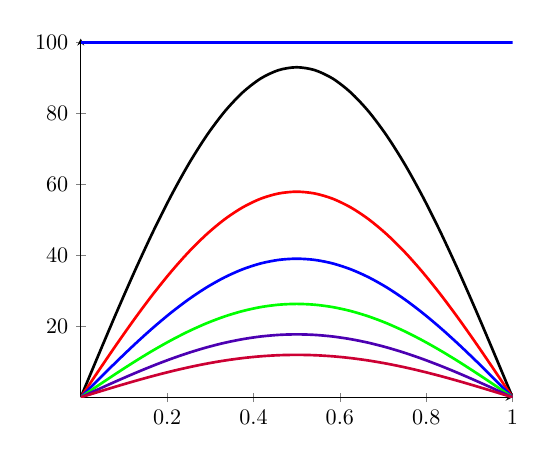
\begin{tikzpicture}[scale=0.8]
            \begin{axis}[axis lines=center, xmin=0, xmax=1, ymin=0, ymax=101]
                \addplot[smooth, blue, very thick, domain=0:1] {100+0*x};
                \addplot[smooth, very thick, domain=0:1]
                {(400/3.14)*sin(pi*x*180/pi)*exp(-0.08*(1*3.14)^2*0.4)};
                \addplot[smooth, red, very thick, domain=0:1]
                {(400/3.14)*sin(pi*x*180/pi)*exp(-0.08*(1*3.14)^2*1.0)};
                \addplot[smooth, blue, very thick, domain=0:1]
                {(400/3.14)*sin(pi*x*180/pi)*exp(-0.08*(1*3.14)^2*1.5)};
                \addplot[smooth, green, very thick, domain=0:1]
                {(400/3.14)*sin(pi*x*180/pi)*exp(-0.08*(1*3.14)^2*2.0)};
                \addplot[smooth, red!30!blue, very thick, domain=0:1]
                {(400/3.14)*sin(pi*x*180/pi)*exp(-0.08*(1*3.14)^2*2.5)};
                \addplot[smooth, red!80!blue, very thick, domain=0:1]
                {(400/3.14)*sin(pi*x*180/pi)*exp(-0.08*(1*3.14)^2*3.0)};
            \end{axis}
        \end{tikzpicture}
    \end{center}
    \caption{Snapshots of the solution to Example \ref{ex:1Dheat_Dirichlet}.}
    \label{fig:example_IC100}
\end{figure}


\subsubsection{Summary of Separation of Variables}
The following steps were used throughout the last several problems to solve a linear
homogeneous PDE with linear and homogeneous boundary conditions.
\begin{enumerate}
    \item Temporarily ignore the initial condition.
    \item Separate the variables by assuming that $u(x,t) = G(t) \phi(x)$.
        \begin{enumerate}
            \item Rearrange the PDE to separate the functions $G$ and $\phi$.
            \item Introduce a separation constant $-\lambda$.
            \item Write the two separate ODEs as eigenvalue problems.
        \end{enumerate}
    \item Determine the separation constants as eigenvalues of a boundary value problem.
    \item Solve the other differential equations.  Record all products of solutions of the
        PDE obtainable by this method.
    \item Apply the principle of superposition: the general solution is a linear
        combination of all of the individual solutions.
    \item Satisfy the initial conditions:
        \begin{enumerate}
            \item substitute $t=0$ into the general solution
            \item multiply both sides of the resulting equation by an appropriate function
                (it should be another basis function from the same vector space that
                builds the infinite sum)
            \item integrate and take advantage of orthogonality
            \item use the resulting integrals to find a pattern in the coefficients.
        \end{enumerate}
    \item Use software to plot the solutions as they evolve over time.
\end{enumerate}

Now it is your turn.  The following two problems allow you to put these ideas to the test.
\begin{problem}
    Solve the 1D heat equation 
    \[ \pd{u}{t} = k \pdd{u}{x} \]
    subject to the boundary conditions $u(0,t) = u(1,t) = 0$ with initial temperature
    profile $u(x,0) = 6\sin(9 \pi x)$.  Start by making a sketch of several time steps of
    the solution using what you now about the physics of the problem.
\end{problem}

\begin{problem}
    Solve the 1D heat equation 
    \[ \pd{u}{t} = k \pdd{u}{x} \]
    subject to the boundary conditions $u(0,t) = u(1,t) = 0$ with initial temperature
    profile $u(x,0) = x(1-x)$.  Start by making a sketch of several time steps of
    the solution using what you now about the physics of the problem.
\end{problem}

\begin{problem}
    So far you have noticed that the spatial differential equation in $\phi$ turns out to
    be an eigenvalue problem 
    \[ \frac{d^2 \phi}{dx^2} = -\lambda \phi.\]
    Determine the eigenvalues of the problem with the following sets of boundary
    conditions:
    \begin{enumerate}
        \item[(a)] $\phi(0) = 0$ and $\phi(\pi) = 0$
        \item[(b)] $\phi(0) = 0$ and $\phi(1) = 0$
        \item[(c)] $\frac{d\phi}{dx}(0) = 0$ and $\frac{d\phi}{dx}(1) = 0$
        \item[(d)] $\phi(0) = 0$ and $\frac{d\phi}{dx}(1) = 0$
    \end{enumerate}
    Each of these relates to a physical problem, so now go back through problems (a) - (d)
    and express each problem as boundary conditions for a 1D heat conducting rod.  What do
    these boundary conditions mean physically (i.e. how are we controlling the heat at the
    ends of the rod)?
\end{problem}

\begin{problem}
    Solve the heat equation with homogenous boundary conditions on a rod of unit length
    with initial condition
    \[ u(x,0) = \left\{ \begin{array}{ll} 0, & 0 < x < 1/3 \\ 100, & 1/3 < x < 2/3 \\ 0,
        & 2/3 < x < 1 \end{array} \right. \]
\end{problem}

\subsection{1D Heat Equation with Insulated Ends}
In this section we consider the heat equation again, but this time we consider the problem
where the ends are insulated instead of being held at a fixed temperature.  In Figure
\ref{fig:1Dheat_rod_Neumann} we see that we are now not letting heat escape from the rod
through the ends.  This means that the energy within the rod from the initial condition
will remain in the rod, but may spread out over time.  
\begin{figure}[ht!]
    \begin{center}
        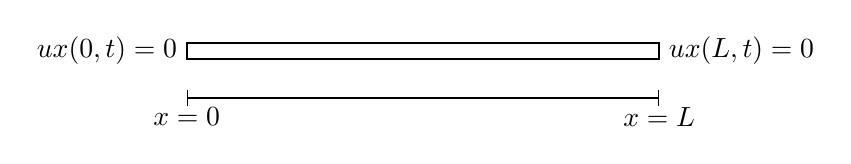
\begin{tikzpicture}
            \draw[thick, black] (0,0) -- (6,0) -- (6,0.2) -- (0,0.2) -- cycle;
            \draw[|-|] (0,-0.5) node[anchor=north]{$x=0$} -- (6,-0.5)
            node[anchor=north]{$x=L$};
            \draw (0,0.1) node[anchor=east]{$\pd{u}{x}(0,t)=0$};
            \draw (6,0.1) node[anchor=west]{$\pd{u}{x}(L,t)=0$};
        \end{tikzpicture}
    \end{center}
    \caption{Sample geometry for the 1D heat equation \eqref{eqn:1Dheat} with Neumann
(insulating) boundary conditions.}
    \label{fig:1Dheat_rod_Neumann}
\end{figure}

As you will soon see, the series solution will actually be in terms of cosines this time
instead of sines.  You will need the following identity:
\begin{flalign}
    \boxed{\int_0^L \cos \left( \frac{n \pi x}{L} \right) \cos\left( \frac{m \pi x}{L} \right) dx
    = \left\{ \begin{array}{ll} 0, & n \ne m \\ \frac{L}{2}, & n = m \ne 0 \\ L, & n=m=0
    \end{array} \right. }
    \label{eqn:cosine_orth}
\end{flalign}

\begin{problem}
    Solve the following 1D heat equation with Neumann boundary conditions.
    \begin{flalign*}
        \pd{u}{t} &= k \pdd{u}{x} \quad \text{ with } t>0 \text{ and } 0 < x < 1 \\
        k &= 1 \quad \text{(this is called the thermal diffusivity)} \\
        \pd{u}{x}(0,t) &= 0 \quad \text{for } t>0 \\
        \pd{u}{x}(L,t) &= 0 \quad \text{for } t>0 \\
        u(x,0) &= -\cos(2\pi x) + 1 \quad \text{for } 0 < x < 1.
    \end{flalign*}
    Start by sketching plots of the time evolution of the initial condition based solely
    on your physical intuition. Then follow the steps for solving a 1D PDE with separation
    of variables.
\end{problem}



\subsection{Heat Equation on a Thin Ring}
Now it is time for a new geometry.  Let us formulate the appropriate initial boundary
value problem for a thin wire (with lateral sides insulated) that is bent into the shape
of a circle.  We will let the wire have length $2L$ as shown in Figure
\ref{fig:1Dheat_ring}. If the wire is thin enough then it is reasonable to assume that the
temperature in the wire is constant along cross sections.  
\begin{figure}[ht!]
    \begin{center}
        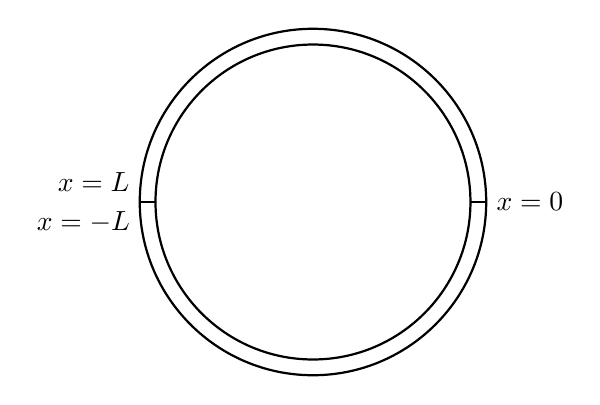
\begin{tikzpicture}
            \draw[thick, black] (0,0) circle(2cm);
            \draw[thick, black] (0,0) circle(2.2cm);
            \draw[thick, black] (-2,0) -- (-2.2,0) node[anchor=south east]{$x=L$};
            \draw[thick, black] (2,0) -- (2.2,0) node[anchor=west]{$x=0$};
            \draw (-2.2,0) node[anchor=north east]{$x=-L$};
        \end{tikzpicture}
    \end{center}
    \caption{A thin circular wire of length $2L$.}
    \label{fig:1Dheat_ring}
\end{figure}

The formulation for the heat equation in this case is:
\begin{flalign*}
    \pd{u}{t} &= k \pdd{u}{x} \quad \text{ with } t>0 \text{ and } -L < x < L \\
    u(-L,t) &= u(L,t) \quad \text{(since the heat must match at $x=\pm L$)} \\
    \pd{u}{x}(-L,t) &= \pd{u}{x}(L,t) \quad \text{(since the derivative of the temp.
    must be continuous)} \\
    u(x,0) &= f(x) \quad \text{for } -L < x < L.
\end{flalign*}

\begin{problem}
    After separating the variables we again have the eigenvalue problem
    \[ \frac{d^2 \phi}{dx^2} = -\lambda \phi. \]
    Choose the proper boundary conditions on this problem?
    \begin{itemize}
        \item[(a)] $\phi(-L) = \phi(L)=0$ and $\frac{d\phi}{dx}(-L) =
            \frac{d\phi}{dx}(L)=0$
        \item[(b)] $\phi(-L) = \phi(L)$ and $\frac{d\phi}{dx}(-L) = \frac{d\phi}{dx}(L)$
        \item[(c)] $\phi(-L) + \phi(L)=0$ and $\frac{d\phi}{dx}(-L) +
            \frac{d\phi}{dx}(L)=0$
        \item[(d)] The moon is made of cheese
    \end{itemize}
\end{problem}


\begin{problem}
    Solve the boundary value problem 
    \[ \frac{d^2 \phi}{dx^2} = -\lambda \phi \]
    with the boundary conditions from the previous voting question. If you get multiple
    solutions (hint) then remember that your final solution is actually a linear
    combination of the solutions.
\end{problem}

\begin{problem}
    The time problem $G(t)$ has the same solutions on a ring as it does for the 1D rod.
    Using this information as well as your solution to the spatial boundary value problem,
    write the full general solution to the heat equation on a thin ring.
\end{problem}

For the heat equation on a ring you should have found that the general solution is
\begin{flalign}
    u(x,t) &= A_0 + \sum_{n=1}^\infty \left[ e^{-k(n\pi/L)^2t} \left( A_n \cos\left(
        \frac{n \pi x}{L}
        \right) + B_n \sin\left( \frac{n \pi x}{L} \right) \right) \right], \quad
        \text{with} 
    \label{eqn:1Dheat_ring_soln}\\
    u(x,0) = f(x) &= A_0 + \sum_{n=1}^\infty \left[ A_n \cos\left( \frac{n\pi x}{L} \right) + B_n
        \sin\left( \frac{n\pi x}{L} \right) \right]
\end{flalign}
In order to find the coefficients we need the following orthogonality identities:
\begin{flalign}
    \int_{-L}^L \cos\left( \frac{n\pi x}{L} \right) \cos\left( \frac{m\pi x}{L} \right) &=
    \left\{ \begin{array}{ll} 0, & n \ne m \\ L, & n = m \ne 0 \\ 2L, & n=m=0 \end{array}
        \right. \\
        \int_{-L}^L \sin\left( \frac{n\pi x}{L} \right) \sin\left( \frac{m \pi x}{L}
        \right) dx &=\left\{ \begin{array}{ll} 0, & n\ne m \\ L, & n=m \ne 0 \end{array}
            \right. \\
        \int_{-L}^L \sin\left( \frac{n\pi x}{L} \right) \cos\left( \frac{m \pi x}{L}
        \right) dx &= 0 \text{ for all $n$ and $m$.}
\end{flalign}

\begin{problem}
    Let's take a ring with $L = 1$ and $f(x) = \sin(2 \pi x)$.  
    \begin{itemize}
        \item Find the coefficients $A_n$ by multiply by $\cos\left( \frac{m\pi x}{1}
            \right)$ and integrating from $-1$ to $1$.
        \item Find the coefficients $B_n$ by multiply by $\sin\left( \frac{m\pi x}{1}
            \right)$ and integrating from $-1$ to $1$.
    \end{itemize}
    You are welcome to use technology to evaluate the integrals.  If you can't get an
    exact formula for the patterns in $A_n$ and $B_n$ at least write down the first 8 or
    10 terms of each sequence.
\end{problem}

\begin{problem}
    For the ring in the last problem with $L=1$ and $f(x) = \sin(2\pi x)$, write down
    several terms in the solution and use technology to make a plot of the time evolution.
    You should start by hand-sketching a plot showing the time evolution of the heat.
\end{problem}



\newpage\section{The Wave Equation (INCOMPLETE)}
This section is incomplete. If I ever get here in MA334 I will finish this section \dots
until then it is going to remain a work in progress.
\[ u_{tt} = \alpha^2 u_{xx} \]
\ldots stuff about waves and such \ldots


\newpage\section{1D Traveling Waves (INCOMPLETE)}
\begin{problem}
    Let $f(x) = e^{-x^2/0.5}$.  Write computer code to animate the function $u(t,x) =
    f(x-at)$ for various values of $a$ on the domain $x \in (-5,5)$.
\end{problem}
% \solution{
% clear; clc; clf;
% f = @(x) exp(-x.^2 / 0.5);
% a = 1;
% u = @(t,x) f(x-a*t);
% x = -5:0.001:5;
% t = 0:0.001:5;
% for n = 1:length(t)
%     plot(x,u(t(n),x),'b')
%     drawnow
% end    
% }

\begin{problem}
    Let $f(x)$ be a function and define $u(t,x)$ be defined as $u(t,x) = f(x-at)$.  
    \begin{enumerate}
        \item[(a)] Find $\ds \pd{u}{t}$
        \item[(b)] Find $\ds \pd{u}{x}$
        \item[(c)] What differential equation does $u(t,x)$ satisfy?
    \end{enumerate}
\end{problem}
\solution{
    \[ u_t = -a u_x \]
}

\begin{problem}
    Solve the differential equation $u_t + 3u_x=0$ with initial condition $u(0,x) = \sin(x)$
    on the domain $x \in [0,2\pi]$ with boundary condition $u(t,0) = 0$.
\end{problem}
\solution{
    \[ u(t,x) = \sin(x-3t) \]
}

The differential equation
\[ u_{t} = -\alpha u_{x} \]
exhibits traveling wave type solutions.
\ldots
General solution is \ldots
\[ u_t + \alpha u_x = 0 \quad \text{with} \quad u(0,x) = \eta(x) \quad \implies \quad
    u(t,x) = \eta(x-\alpha t) \]
since by the chain rule 
\[ u_t + \alpha u_x = \pd{ }{t} \left( \eta(x-\alpha t) \right) + \alpha \pd{ }{x} \left(
    \eta(x-\alpha t) \right)=
    -\alpha \eta(x-\alpha t) + \alpha \eta(x-\alpha t) = 0. \]

\newpage\section{Additional Exercises}

\newpage
\begin{center}
    {\LARGE The End}
\end{center}
\newpage



